\chapter{Instalación}
\label{ch:guia}


La instalación puede parecer un poco repetitiva pero la idea es que cada parte del producto final se ejecute en un Docker independiente (ver detalles más adelante), así que, en esta sección se pretende explicar los requerimientos necesarios para cada una de las partes y después hacer una breve guía de uso de las mismas.

\section{Instalación procesamiento de texto}

La instalación del paquete para el procesamiento de texto en Ubuntu es bastante simple. Se requiere instalar \texttt{Python}, \texttt{R} y algunas pocas librerías de \texttt{Python} usando \texttt{apt-get} y las demás se instalan solas al instalar la librería \texttt{itm}. Cabe mencionar que el proceso puede correr incluso si no están instaladas correctamente todas las dependencias, pero los procesos que las utilicen fallarán.

\begin{lstlisting}
 
# Necesario para instalar R >= 3.1
echo "deb http://cran.rstudio.com/bin/linux/ubuntu trusty/" >> /etc/apt/sources.list && \
	sudo apt-key adv --keyserver keyserver.ubuntu.com --recv-keys E084DAB9

# Actualizar indices de apt-get
sudo apt-get update && \
	apt-get upgrade # Necesario para instalar R >= 3.1

# Instalar Python	2.7 y PyPi
sudo apt-get install -y \
	python2.7-dev \
	python-pip

# Instalar R (debe ser >= 3.1)
sudo apt-get install -y \
	r-base \
	r-base-dev && \
	R --version

# Librerias de algebra lineal, Fortran y compilador de Markdown
sudo apt-get install -y \
	libblas-dev \
	liblapack-dev \
	gfortran \
	pandoc

# Instalar el paquete itm	y sus dependencias de Python
PACK = /ruta/a/paquete/itm-a.b # Donde a.b es la versi\'on (ej: itm-0.3)
pip install $PACK

# Instalar librerias de R y bajar stopwords de nltk (no se bajan al bajar el paquete)
R -e 'install.packages(c("dplyr", "optparse", "networkD3"), repos = "http://cran.us.r-project.org")'
python -c "import nltk; nltk.download('stopwords')"
\end{lstlisting}


\section{Instalación procesamiento de imágenes}

\begin{lstlisting}
#Instalar R

sudo sh -c 'echo "deb http://cran.rstudio.com/bin/linux/ubuntu trusty/" \
>> /etc/apt/sources.list'

gpg --keyserver keyserver.ubuntu.com --recv-key E084DAB9
gpg -a --export E084DAB9 | sudo apt-key add -

sudo apt-get update
sudo apt-get -y install r-base

#Instalar paquetes
sudo su - -c "R -e \"install.packages('dplyr', \
repos='http://cran.rstudio.com/', dependencies = TRUE)\""
sudo su - -c "R -e \"install.packages('jpeg',\
repos='http://cran.rstudio.com/', dependencies = TRUE)\""
sudo su - -c "R -e \"install.packages('lsa', \
repos='http://cran.rstudio.com/')\""

##Instalar paquetes python

sudo apt-get install python-numpy python-scipy \
python-matplotlib ipython ipython-notebook \
python-pandas python-sympy python-nose \
python-skimage

sudo apt-get install python-pip
sudo pip install -U scikit-learn


#Instalar luigi

wget https://pypi.python.org/packages/source/l/luigi/luigi-2.0.0.tar.gz#md5=06258afcfcdd2f829167450fd5fed604
tar -xzvf luigi-2.0.0.tar.gz
cd luigi-2.0.0/
sudo python setup.py install

#instalar imagemagick
sudo apt-get install imagemagick

##Instalar tornado para que funcione el central scheduler
wget https://pypi.python.org/packages/source/t/tornado/tornado-4.3.tar.gz
tar -xzvf tornado-4.3.tar.gz
cd tornado-4.3
python setup.py install

##Copio los scripts a mi instancia
scp -r Luigi_Imagenes root@ip_instancia:/home
\end{lstlisting}

\section{Instalación para el análisis de logs}

Para la ejecución del pipeline de análisis de Logs es necesario instalar \texttt{Python}, \texttt{R} y bibliotecas de \texttt{Python} usando \texttt{apt-get}


\begin{lstlisting}
# Necesario para instalar R >= 3.1
echo "deb http://cran.rstudio.com/bin/linux/ubuntu trusty/" >> /etc/apt/sources.list && \
	sudo apt-key adv --keyserver keyserver.ubuntu.com --recv-keys E084DAB9

# Actualizar indices de apt-get
sudo apt-get update && \
	apt-get upgrade # Necesario para instalar R >= 3.1

# Instalar R (debe ser >= 3.1)
sudo apt-get install -y \
	r-base \
	r-base-dev && \
	
# Instalar dependencias de R
R -e 'install.packages(c("dplyr", "shiny", "ggplot2"), repos = "http://cran.us.r-project.org")'

# Instalar Python
sudo apt-get install build-essential checkinstall

sudo apt-get install libreadline-gplv2-dev libncursesw5-dev \
libssl-dev libsqlite3-dev tk-dev libgdbm-dev libc6-dev libbz2-dev

sudo apt-get install python2.7

# Instalar dependencias de Python

sudo pip install luigi
sudo apt-get install python-matplotlib
\end{lstlisting}

\section{Instalación Docker}

Para facilitar la instalación anterior se decidió instalar una máquina virtual por medio de Docker, un servicio para administrar Máquinas Virtuales. Docker facilita la instalación y hace la copia de las máquinas un proceso muy simple. El objetivo es poder ejecutar aplicaciones tan complejas como sea necesario en cualquier lugar de una manera sencilla. Los servicios en la nube como Amazon utilizan esta herramienta para poder montar aplicaciones por medio de máquinas virtuales fáciles de preparar.

Para instalar Docker en Ubuntu se siguió las sugerencias de la página \href{http://docs.docker.com/engine/installation/ubuntulinux/}{Instalación Docker}. Es decir, basta con ejecutar los siguientes comandos:

\begin{lstlisting}
# Actualizar apt-get
sudo apt-get update

# Instalar el paquete recomendado
sudo apt-get install linux-image-extra-$(uname -r)

# Instalar Docker
sudo apt-get install docker-engine

# Empezar el servidor
sudo service docker start

# Correr una maquina virtual
# NOTA este comando descarga una imagen con Ubuntu
sudo docker run ubuntu
\end{lstlisting}

Una vez instalado Docker,  se puede descargar la siguiente imagen de una máquina virtual que contiene los paquetes necesarios para ejecutar el procesamiento de imágenes y de texto junto con el análisis de logs.

\begin{lstlisting}
# Descarga la maquina con el procesamiento de texto
sudo docker pull carpetri/itam_tm:v0.3

# Descarga la maquina con el procesamiento de imagenes
sudo docker pull jared275/luigimage
\end{lstlisting}


%FALTA PONER LA MAQUINA DE LOGS

\section{Breve guía de uso}
\subsection{Guía para el procesamiento de texto}

Una vez instalado Docker con  el paquete se puede acceder a los ejecutables desde la consola. Para facilitar su uso se escribieron dos \emph{wrappers}, uno \emph{simple} que sólo pide los parámetros indispensables (\texttt{itam-tm-default}) y otro \emph{avanzado} (\texttt{itam-tm}) que requiere que se especifique todos los parámetros de entrada internos del proceso de \texttt{luigi}. El ejecutable \emph{avanzado} corre un solo proceso a la vez y se debe conocer cómo funciona internamente el paquete, mientras que el \emph{simple} corre todos los análisis para valores especificados de los parámetros.

A continuación se muestra cómo utilizar el \emph{simple} para correr el análisis. Con el fin de probar la instalación y que todo corriera sin problemas, se instaló el paquete en un contenedor de Docker, desde donde se ejecutará todo.

Para empezar hay que ejecutar la máquina virtual que contiene el Docker de procesamiento de texto con el siguiente comando:


 Notar que la bandera \-p es para el puerto. La bandera \-v es para poder ver la carpeta con los libros (en este caso ITAM). Además es importante porque aquí será donde se verán los resultados.
\begin{lstlisting}
sudo docker run -it --name proceso_texto -p 8082:8082 -v /home/dspaceadmin/ITAM/:/home/itam/ carpetri/itam_tm:v0.3 /bin/bash

\end{lstlisting}

Se empieza con una carpeta \texttt{test} en donde están los datos crudos:

\begin{lstlisting}
root@7351c9042a96:/home/itam# ls -lh test
total 0
drwxr-xr-x 1 1000 staff 340 Oct 27 01:49 jpg
drwxr-xr-x 1 1000 staff 340 Nov  3 22:32 pdf
root@7351c9042a96:/home/itam# ls -lh test/pdf/
total 0
drwxr-xr-x 1 1000 staff  748 Oct 27 01:49 1200_years_of_italian_sculpture
drwxr-xr-x 1 1000 staff  680 Oct 27 01:49 12_dibujos_de_jose_maria_velasco
drwxr-xr-x 1 1000 staff 2.8K Oct 27 01:49 20_dibujos_mexicanos_de_maroto
drwxr-xr-x 1 1000 staff 2.5K Oct 27 01:49 revue_des_peintres
drwxr-xr-x 1 1000 staff  952 Oct 27 01:49 tehuantepec
drwxr-xr-x 1 1000 staff 1.8K Oct 27 01:49 vitral
drwxr-xr-x 1 1000 staff  884 Oct 27 01:49 zuniga
drwxr-xr-x 1 1000 staff  918 Oct 27 01:50 zurbaran
root@7351c9042a96:/home/itam# ls -lh test/pdf/zuniga/
total 12M
-rw-r--r-- 1 1000 staff 278K Oct 27 01:49 zun-ctp_00000001.pdf
-rw-r--r-- 1 1000 staff 261K Oct 27 01:49 zun-int_00000001.pdf
-rw-r--r-- 1 1000 staff 168K Oct 27 01:49 zun-int_00000002.pdf
-rw-r--r-- 1 1000 staff 208K Oct 27 01:49 zun-int_00000003.pdf
-rw-r--r-- 1 1000 staff 164K Oct 27 01:49 zun-int_00000004.pdf
-rw-r--r-- 1 1000 staff 139K Oct 27 01:49 zun-int_00000005.pdf
\end{lstlisting}

El siguiente paso es inicializar el servidor de \texttt{luigi}, con el comando siguiente (o alternativamente, se puede agregar \texttt{--local-sceduler} al llamar \texttt{itam-tm-default}):

\begin{lstlisting}
root@7351c9042a96:/home/itam# luigid --background &
\end{lstlisting}

Lo anterior deja el servidor corriendo en segundo plano de manera silenciosa. En la dirección IP `8082` \texttt{luigi} genera un dashboard desde el cual se puede ver el avance. Se puede acceder a él desde un navegador yendo a la dirección \texttt{localhost:8082}. Ya con eso andando sólo es necesario correr el siguiente comando (parámetros de ejemplo):

\begin{lstlisting}
root@7351c9042a96:/home/itam# itam-tm-default \
  -d test \
  --identifier prueba \
  --no-timestamp \
  --languages spanish,english \
  --clean-level clean,stopwords
  --topic-range-lda 3,10,2 \
  --topic-range-lsi 40,81,20 \
  --workers 6
\end{lstlisting}

Los parámetros equivalen a lo siguiente:
\begin{itemize}

\item \texttt{-d, --root-directory [ruta/maestra]} es la ruta que contiene la carpeta \texttt{pdf}.

\item \texttt{--languages idioma1[,idioma2[,...]]} son los idiomas a procesar. Hay que notar que siempre se limpian todos los textos que no hayan sido procesados antes. Esta bandera afecta desde la creación del diccionario y el corpus en adelante.
\item  \texttt{-i, --indentifier [nombre]} le pone el sufijo `nombre` a las carpetas de modelos y resultados con el \item  \texttt{[--no-timestamp]} no poner \textbf{timestamp} en el nombre de las carpetas de modelos y resultados después del identificador.
\item \texttt{[--no-md5]} no revisar las sumas MD5 de los PDFs de entrada ni ponerla en el nombre de las carpetas de modelos y resultados después del \textbf{timestamp} (si hay).
\item \texttt{--clean-level (raw|clean|stopwords)[,(raw|clean|stopwords)[,...]]} agrega los niveles de limpieza a procesar y a modelar.
\item  \texttt{--topic-range-lda start,stop+1,step} hace un modelo LDA para cada nivel de limpieza y para cada número de tópicos, para `start, start + step, ..., stop`.
\item \texttt{--topic-range-lsi start,stop+1,step} hace un modelo LSI para cada nivel de limpieza y para cada número de tópicos, para `start, start + step, ..., stop`.
\item  \texttt{--workers n} lleva a cabo el proceso de extracción y limpieza con \texttt{n} procesos en paralelo.

\end{itemize}

Una vez corriendo lo anterior, el dashboard se ve, por ejemplo, como en la figura (\ref{fig:luigi-dashboard}), qué procesos están corriendo, han sido terminados o faltan por correr. También se puede filtrar los procesos y ver sus árboles de dependencias entre otras cosas.

\begin{figure}[H]
\centering
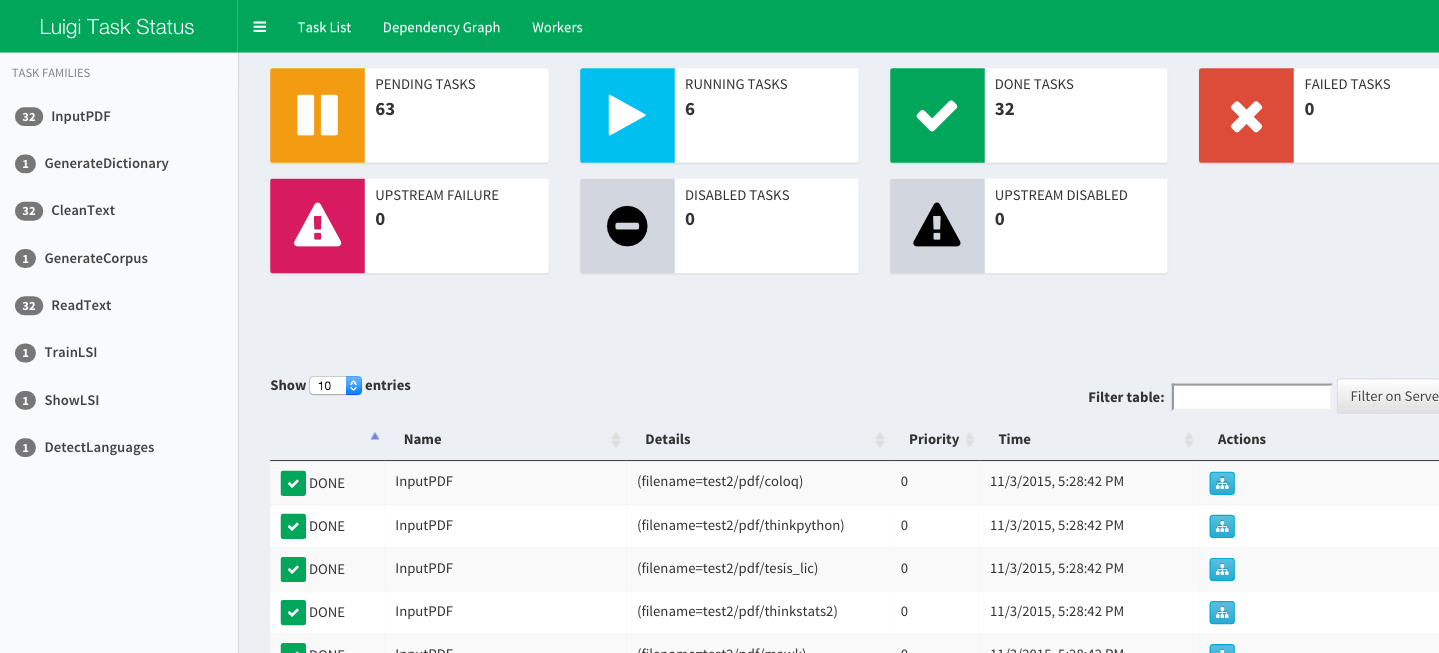
\includegraphics[width=1\textwidth]{Figures/dashboard.png}
\caption{Dashboard de \texttt{luigi} corriendo en el navegador.\label{fig:luigi-dashboard}}
\end{figure}


El dashboard provee muchas formas prácticas para filtrar las tareas, según si están corriendo (azul), si terminaron (verde), si tuvieron algún problema (rojo) o si están pendientes (amarillo). Se puede ver también la información más relevante, como qué proceso está corriendo y con qué parámetros y qué proceso se está encargando de hacerlo. \texttt{Luigi} también proporciona una vista de red, en la que se puede ver gráficamente el árbol de dependencias, como se puede ver en la figura (\ref{fig:lsi-tree}).

\begin{figure}[H]
\centering
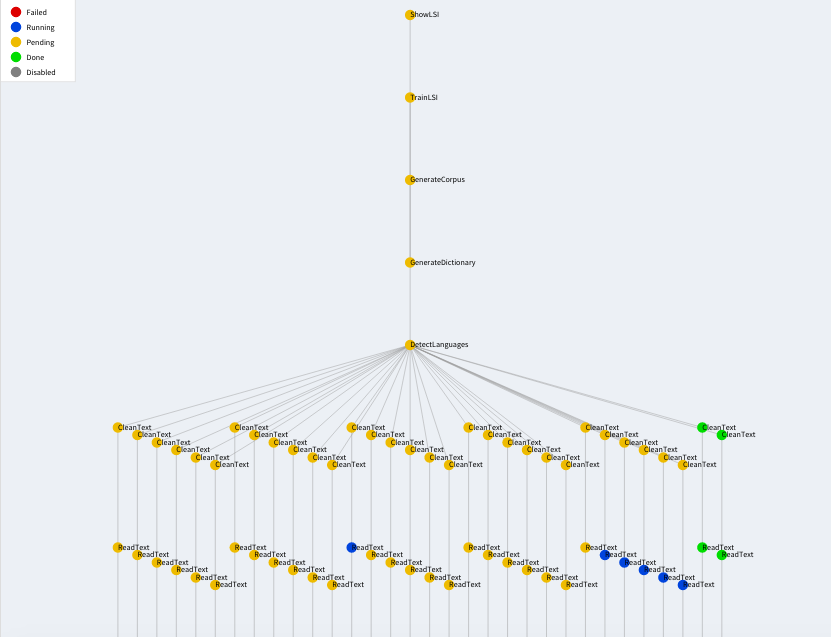
\includegraphics[width=1\textwidth]{Figures/detail.png}
\caption{Árbol de dependencias del LSI con seis procesos corriendo en paralelo.\label{fig:lsi-tree}}
\end{figure}


Con la gráfica es fácil ilustrar algunas de las ventajas del orquestador. Por ejemplo, si se agregan dos libros a la colección, sólo corren los procesos que son estrictamente necesarios (aquí, los modelos, etc.), pero no la limpieza que ya haya sido ejecutada, ya que  \texttt{Luigi} detecta automáticamente qué hay que correr y qué ya no es necesario. En la figura (\ref{fig:luigi-parallel}) se ejemplifica esto.


\begin{figure}[H]
\centering
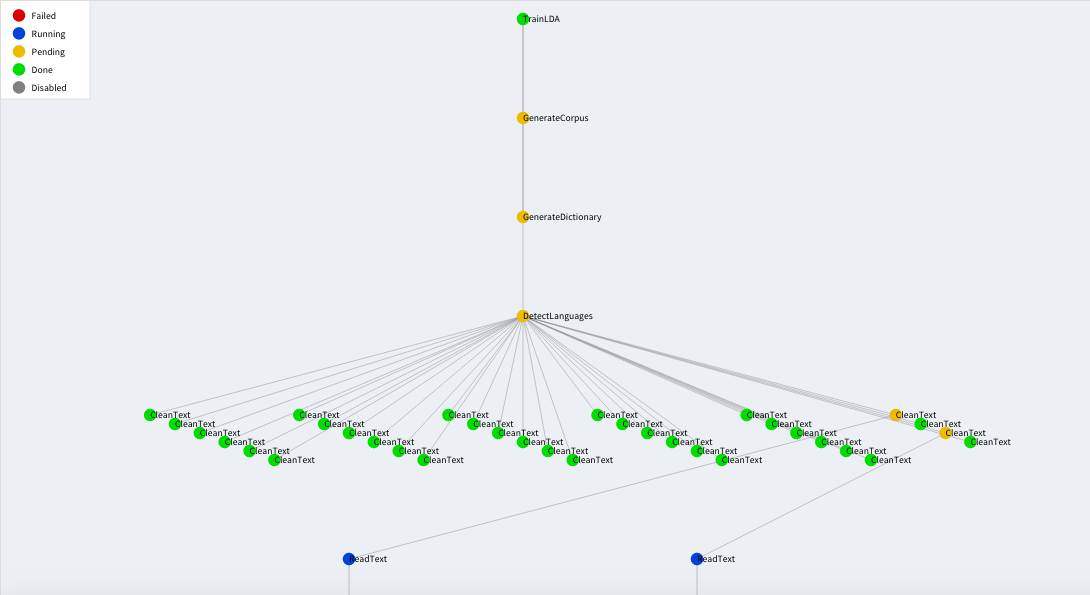
\includegraphics[width=1\textwidth]{Figures/detail2.png}
\caption{Árbol de dependencias del LSI con dos libros que no habían sido procesados.\label{fig:luigi-parallel}}
\end{figure}

\subsection{Guía para  el procesamiento de imagen}

Para empezar hay que ejecutar la máquina virtual que contiene el Docker de procesamiento de imágenes con el siguiente comando:


\# Notar que la bandera \-p es para el puerto. La bandera \-v es para poder ver la carpeta con los libros (en este caso ITAM). Además es importante porque aquí sera donde se verán los resultados.
\begin{lstlisting}
sudo docker run -it --name proceso_imagenes -p 8082:8082 -v /home/dspaceadmin/ITAM/:/home/itam/ jared275/luigimage /bin/bash
\end{lstlisting}

Se decidió realizar pruebas antes de correr el proceso sobre todas las imágenes, por lo que se colectaron 100 libros aleatorios que se guardaron en \texttt{/home/dspaceadmin/ITAM/Libros\_prueba}.

El proceso por el cual se escogieron los 100 libros de manera aleatoria se hizo con el siguiente script:

\begin{lstlisting}
ls /export/librarian | sort --random-sort | head -100 | parallel 'cp -r /export/librarian/{} /home/dspaceadmin/ITAM/Libros_prueba/'
\end{lstlisting}

Con lo anterior ya se puede entrar a la máquina con el procesamiento de imágenes con el comando 

\begin{lstlisting}
sudo docker start -ia proceso_imagen_prueba
\end{lstlisting}

Una vez dentro del Docker se pueden ver  los 100 libros de prueba con la salida:

\begin{lstlisting}
root@18e42a789d4f:/home/itam# ls -la Libros/        
total 408
drwxrwxr-x 102 1000 1000 4096 Nov 21 19:37 .
drwxr-xr-x  16 root root 4096 Dec  2 17:45 ..
drwxrwxr-x   4 1000 1000 4096 Nov 21 19:33 alfredo_zalce_artista
drwxrwxr-x   4 1000 1000 4096 Nov 21 19:31 antonio_ruiz_el_corcito
drwxrwxr-x   4 1000 1000 4096 Nov 21 19:27 biblioteca_de_chapulin
drwxrwxr-x   4 1000 1000 4096 Nov 21 19:30 blanco_y_negro_revista_ilustrada_7_de_abril_de_1918_n._1.403
drwxrwxr-x   4 1000 1000 4096 Nov 21 19:33 calendario_de_galvan_1843
drwxrwxr-x   4 1000 1000 4096 Nov 21 19:31 calendario_de_galvan_pra_el_ano_de_1841
...
\end{lstlisting}

Ahora se está listo para ejecutar el proceso. Para esto los parámetros a elegir son:

\begin{itemize}
\item \texttt{--directorio-libros}: Una liga que apunte al directorio en donde se encuentran los libros con los jpeg.
\item \texttt{--workers} n: lleva acabo el proceso con $n$ procesos en paralelo.
\end{itemize}

Finalmente para ejecutar el proceso basta con escribir el comando a continuación:

\begin{lstlisting}
cd Luigi_Imagenes
python data_flow_EInfo.py LocalSensitiveHashing --directorio-libros \ /home/itam/Libros --workers 12
\end{lstlisting}

Este proceso tardó aproximadamente 3 horas en correr, por lo que se calcula, si se conservan los tiempos vistos en esta prueba, que correrlo sobre los  3,625 libros tardará aproximadamente 110 horas.

El resultado de este pipeline se puede ver el archivo de similitudes

\begin{lstlisting}
root@18e42a789d4f:/home/itam/Luigi_Imagenes# cat 100_libros_similitudes_paginas.csv  | head -7
"","V1","V2","V3"
"","0.93","connecticut_william_hubbellxxYxxcwh-int_00000054.jpg",
"peintres_du_xx_e_sieclexxYxxpein-dxx-int_00000057.jpg"
"","0.98","ritvale_sacri_et_regalisxxYxxrser-int_00000184.jpg",
"ritvale_sacri_et_regalisxxYxxrser-int_00000440.jpg"
"","0.99","ritvale_sacri_et_regalisxxYxxrser-int_00000323.jpg",
"ritvale_sacri_et_regalisxxYxxrser-int_00000325.jpg"
"","0.97","ritvale_sacri_et_regalisxxYxxrser-int_00000106.jpg",
"ritvale_sacri_et_regalisxxYxxrser-int_00000109.jpg"
"","0.83","cezanne_la_obra_de_una_vidaxxYxxczz-int_00000052.jpg"
,"the_art_of_the_printxxYxxtatp-int_00000065.jpg"
"","0.91","alfredo_zalce_artistaxxYxxaza-int_00000056.jpg",
"cezanne_la_obra_de_una_vidaxxYxxczz-int_00000051.jpg"
\end{lstlisting}

\subsection{Guía para el procesamiento de clickstream}\label{instalacion}


\subsubsection{Breve guía de uso}\label{breve-guia-de-uso}

Una vez instalado lo anterior, se necesitan 3 cosas para ejecutar el
pipeline correctamente, la función \emph{analisis-log-itam.py}, el
archivo \emph{access.log} y la carpeta de \emph{functions} la cuál trae
funciones externas. Lo necesario deberá estar en una ruta especificada
por el usuario.

En la línea de comandos ir hasta la ruta donde se tiene lo anterior

\begin{lstlisting}
#Ejemplo:
  cd User/miruta/misarchivos
  
\end{lstlisting}

Para ejecutar el pipeline y visualizar el proceso es necesario abrir
otra línea de comandos y el navegador

\begin{lstlisting}
#Dentro de la linea de comandos teclear:

  luigid

#Dentro del navegador, abrir el puerto y poner la siguiente direccion:

  http://localhost:8082/static/visualiser/index.html#
\end{lstlisting}

Posteriormente en la línea de comandos (diferente a donde se tecleo
\emph{luigid}), ejecutar la función.

\begin{lstlisting}
python analisis-log-itam.py Enriquecer --input-file access.log --output-file\
usuario.pd  --output-df sesionizar.pd --output-df1 enriquecer --output-df2\
reporte.pd
\end{lstlisting}

La salida que se obtendrá será la siguiente

\begin{lstlisting}
===== Luigi Execution Summary =====

Scheduled 5 tasks of which:
* 1 present dependencies were encountered:
    - 1 Inputlog(filename=access.log)
    
* 4 ran successfully:

    - 1 Sesionizar(input_file=access.log, output_file=usuario.pd,
    output_df=sesionizar.pd, output_df1=enriquecer)
    - 1 Parsear(input_file=access.log, output_file=usuario.pd)
    
    - 1 Enriquecer(input_file=access.log, output_file=usuario.pd,
    output_df=sesionizar.pd, output_df1=enriquecer, output_df2=reporte.pd)
    
    - 1 Usuario(input_file=access.log, output_file=usuario.pd, output_df=sesionizar.pd)

This progress looks :) because there were no failed tasks or
missing external dependencies

===== Luigi Execution Summary =====
\end{lstlisting}

Una vez ejecutado, dentro de la ruta se crearan 5 archivos que son los
outputs descritos con anterioridad \emph{reporte.pd},
\emph{sesionizar.pd}, \emph{usuario.pd} y \emph{enriquecer.csv}

Dentro del navegador que se haya abierto con anterioridad se tendrá la siguiente vista:

\begin{figure}[H]
\centering
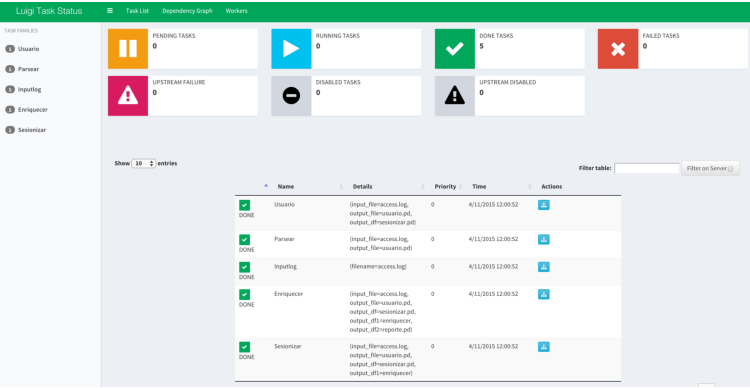
\includegraphics[width=1\textwidth]{Figures/unnamed-chunk-2-1}
\caption{Dashboard de luigi-análisis clickstream}
\end{figure}

\begin{figure}[H]
\centering
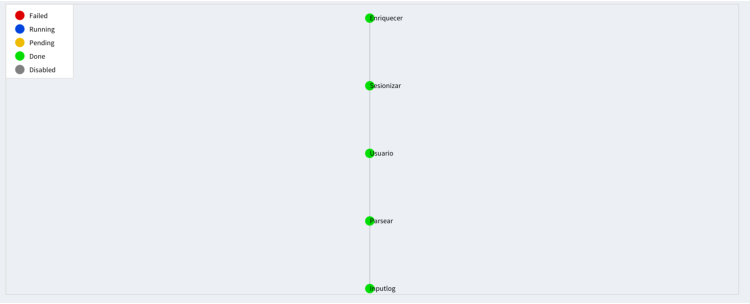
\includegraphics[width=1\textwidth]{Figures/unnamed-chunk-3-1}
\caption{Árbol de dependencias clickstream}
\end{figure}



\subsection{ Ejecución Dashboard}\label{ejecucion-dashboard}

Para poder ejecutar el dashboard es necesario que en la ruta
especificada por el usuario (la cual debe ser la misma donde se
obtuvieron los outputs y el archivo enriquecer.csv), es necesario tener
la carpeta \emph{/R} la cual a su vez tiene dos archivos \emph{server.R}
y \emph{ui.R}

Nuevamente en la línea de comandos, ejecutar:

\begin{lstlisting}
R \-e \textquotedblleft shiny::runApp(\textasciitilde /User/.../R/shinyapp) \textquotedblright
\end{lstlisting}

Al ejecutarse, se tendrá la siguiente salida:

\begin{lstlisting}
> shiny::runApp('~/Desktop/conacyt/R/shinyapp')
Loading required package: shiny
This version of Shiny is designed to work with htmlwidgets >= 0.4. 
Please upgrade your version of htmlwidgets.


Listening on http://127.0.0.1:5127
\end{lstlisting}

El puerto donde se ejecuta el dashboard será el hostname que se muestra,
el cual se tendrá que copiar y pegar en el navegador para poder observar
el dashboard.

Si todo es correcto, se mostrará lo siguiente:

\begin{figure}[H]
\centering
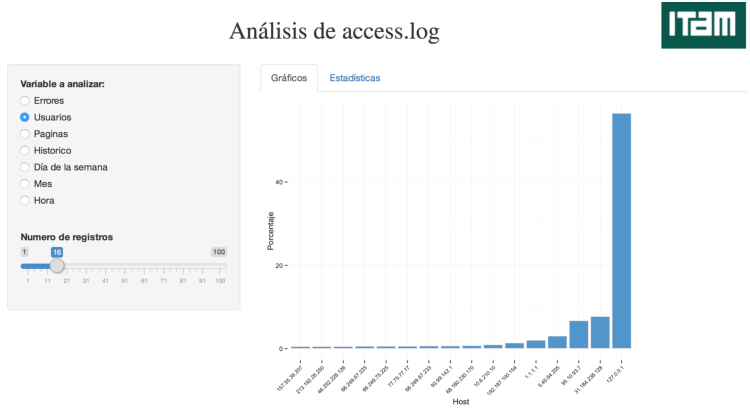
\includegraphics[width=1\textwidth]{Figures/unnamed-chunk-4-1}
\caption{Dashboard  gráficos}
\end{figure}

\begin{figure}[H]
\centering
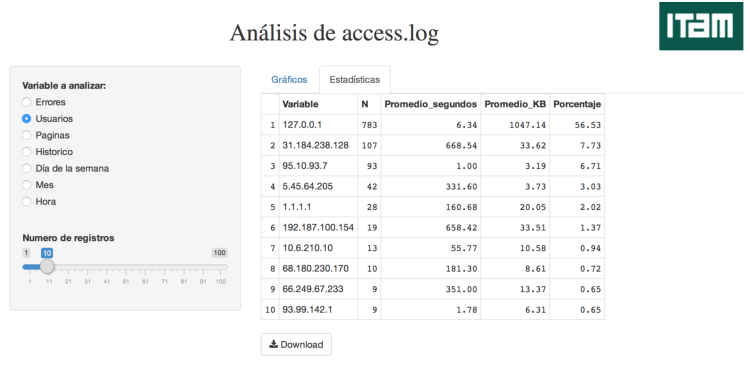
\includegraphics[width=1\textwidth]{Figures/unnamed-chunk-5-1}
\caption{Dashboard  estadísticas}
\end{figure}

En la parte del dashboard, además de poder visualizar las estadísticas
de las variables más importantes, se podrá descargar en formato
\emph{csv} la consulta que le interese al usuario y si esta no le
satisface, podrá descargar los insumos completos.

